\documentclass[12pt]{article}
\usepackage{graphicx}
\usepackage{caption}
\usepackage{geometry}
\usepackage{listings}
\usepackage{amsthm}
\geometry{margin=1in}
\RequirePackage{amsmath}
\usepackage{cite}
\usepackage{amsmath,amssymb,amsfonts,amsthm}
\usepackage{algorithmic}
\usepackage{textcomp}
\usepackage{xcolor}
\usepackage{txfonts}
\usepackage{enumitem}
\usepackage{mathtools}
\usepackage{gensymb}
\usepackage{comment}
\usepackage[breaklinks=true]{hyperref}
\usepackage{tkz-euclide} 
\usepackage{listings}                                                            \usepackage[utf8]{inputenc}     
\usepackage{xparse}
\usepackage{color}                                            
\usepackage{array}                                            
\usepackage{longtable}                                       
\usepackage{calc}                                             
\usepackage{multirow}
\usepackage{multicol}
\usepackage{hhline}                                           
\usepackage{ifthen}                                           
\usepackage{lscape}
\usepackage{tabularx}
\usepackage{array}
\usepackage{float}
\usepackage{gvv}
\usepackage{gvv-book}

\author{EE25BTECH11010-ARSH DHOKE}

\title{GATE 2008 Multiple Choice Questions}
\date{}

\begin{document}

\maketitle

\textbf{Q.1 -- Q.20 Carry one mark each}

\begin{enumerate}
   \item The total number of isomers of Co(en)$_2$Cl$_2$ (en = ethylenediamine) is
   \begin{enumerate}
       \begin{multicols}{2}
         \item 4 
         \item 3 
         \item 6 
         \item 5
    \end{multicols}
    \hfill (GATE CY 2008)
   \end{enumerate}
   

   
    \item   Metal-metal quadruple bonds are well-known for the metal
\begin{enumerate}
\begin{multicols}{2}
\item  Ni 
\item  Co  
\item  Fe  
\item  Re   
\end{multicols} 
\hfill{\brak{\text{GATE CY 2008}}}
\end{enumerate}

    \item The reaction of Al$_4$C$_3$ with water leads to the formation of
   \begin{enumerate}
    \begin{multicols}{2} \item  methane  \item  propyne  \item  propene  \item  propane  \end{multicols}
    \end{enumerate}
\hfill{\brak{\text{GATE CY 2008}}}

 \item The correct statement about C$_{60}$ is
\begin{enumerate}
        \item  C$_{60}$ is soluble in benzene 
        \item  C$_{60}$ does not react with \textit{tert}-butyllithium 
        \item  C$_{60}$ is made up of 10 five–membered and 15 six–membered rings 
        \item  Two adjacent five–membered rings share a common edge
    \hfill (GATE CY 2008)
    \end{enumerate}

\item  The lattice parameters for a monoclinic crystal are
\begin{enumerate}
    \item  $a \neq b \neq c; \ \alpha = \gamma = 90^\degree$
    \item  $a = b \neq c; \ \alpha \neq \beta \neq \gamma$
    \item $a \neq b \neq c; \ \alpha \neq \beta \neq \gamma$\
    \item  $a = b = c; \ \alpha = \gamma = 90^\degree$    \hfill{\brak{\text{GATE CY 2008}}}
\end{enumerate}
    



    \item The magnetic moment of [Ru(H$_2$O)$_6$]$^{2+}$
 corresponds to the presence of
    \begin{enumerate}
    \item  four unpaired electrons 
    \item  three unpaired electrons
    \item  two unpaired electrons 
    \item  zero unpaired electrons    \hfill{\brak{\text{GATE CY 2008}}}
    \end{enumerate}

    

    \item The compound that is \textbf{NOT} aromatic is

\begin{enumerate}
\begin{figure}[H]
    \item 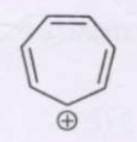
\includegraphics[width=0.1\columnwidth]{figs/q7 a.png}
         \caption{Option A}
    \label{fig:q7 a}
    \item 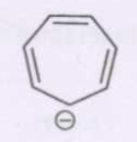
\includegraphics[width=0.1\columnwidth]{figs/q7 b.png}
         \caption{Option B}
    \label{fig:q7 b}
    \item 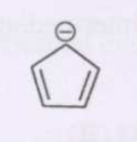
\includegraphics[width=0.1\columnwidth]{figs/q7 c.png}
      \caption{Option C}
    \label{fig:q7 c}
    \item 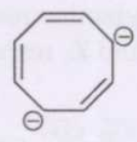
\includegraphics[width=0.1\columnwidth]{figs/q7 d.png}
\caption{Option D}
    \label{fig:q7 d}
    \end{figure}
\end{enumerate}


\bigskip
    \hfill{\brak{\text{GATE CY 2008}}}


\item The order of stability for the following cyclic olefins is

\begin{figure}[H]
  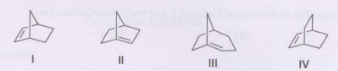
\includegraphics[width=0.7\columnwidth]{figs/q8.png} 
  \caption{Figure for Q.8}
    \label{fig:q8}
\end{figure}

\begin{enumerate}
  \item I \(<\) II \(<\) III \(<\) IV
  \item I \(<\) III \(<\) IV \(<\) I
  \item II \(<\) III \(<\) I \(<\) IV
  \item IV \(<\) II \(<\) I \(<\) III
\end{enumerate}    \hfill{\brak{\text{GATE CY 2008}}}


\item The most acidic species is

\begin{enumerate}
\begin{figure}[H]
    \item 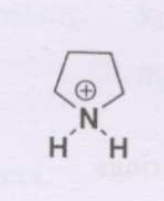
\includegraphics[width=0.1\columnwidth]{figs/q9 a.png} 
     \caption{Option A}
    \label{fig:q9 a}
    \item 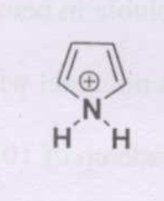
\includegraphics[width=0.1\columnwidth]{figs/q9 b.png} 
    \caption{Option B}
    \label{fig:q9 b}
    \item 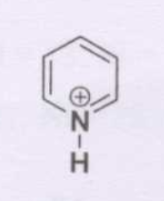
\includegraphics[width=0.1\columnwidth]{figs/q9 c.png}
    \caption{Option C}
    \label{fig:q9 c}
    \item 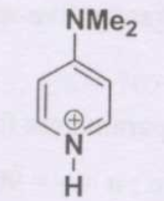
\includegraphics[width=0.1\columnwidth]{figs/q9 d.png} 
    \caption{Option D}
    \label{fig:q9 d}
    \end{figure}
\end{enumerate}
   \hfill{\brak{\text{GATE CY 2008}}}




\item The major product of the following reaction is

\begin{figure}[H]
  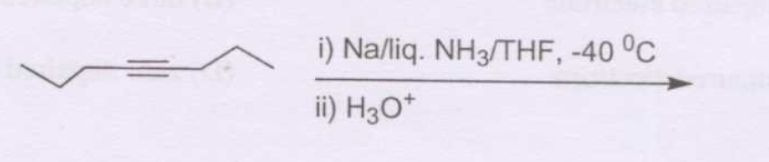
\includegraphics[width=0.7\columnwidth]{figs/q10.png} 
  \caption{Figure for Q.10}
    \label{fig:q10}
      \end{figure}
\begin{enumerate}
  \begin{figure}[H]
    \item 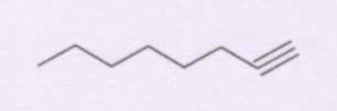
\includegraphics[width=0.3\columnwidth]{figs/q10 a.png}
     \caption{Option A}
    \label{fig:q10 a}
    \item 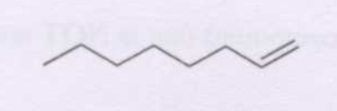
\includegraphics[width=0.3\columnwidth]{figs/q10 b.png}
     \caption{Option B}
    \label{fig:q10 b}
    \item 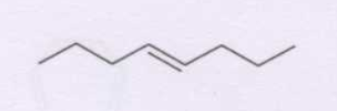
\includegraphics[width=0.3\columnwidth]{figs/q10 c.png}
     \caption{Option C}
    \label{fig:q10 c}
    \item 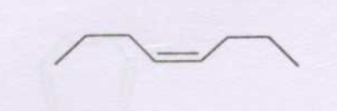
\includegraphics[width=0.3\columnwidth]{figs/q10 d.png}
     \caption{Option D}
    \label{fig:q10 d}
    \end{figure}
\end{enumerate}
\hfill{\brak{\text{GATE CY 2008}}}


 

\item In the carbylamine reaction, R–X is converted to R–Y \textit{via} the intermediate Z.
R–X, R–Y and Z, respectively, are
\begin{enumerate}
    \item R–NH$_2$, R–NC, carbene
    \item R–NH$_2$, R–NC, nitrene
    \item R–NC, R–NH$_2$, carbene
    \item R–OH, R–NC, nitrene     \hfill{\brak{\text{GATE CY 2008}}}
\end{enumerate}
    

    

   \item  The compound that is \textbf{NOT} oxidized by KMnO$_4$ is
\begin{enumerate}
 \begin{figure}[H]
     \item 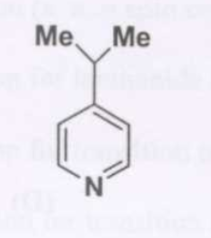
\includegraphics[width=0.1\columnwidth]{figs/q12 a.png}
     \caption{Option A}
    \label{fig:q12 a}
     \item 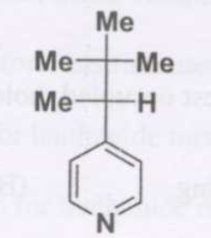
\includegraphics[width=0.1\columnwidth]{figs/q12 b.png}
      \caption{Option B}
    \label{fig:q12 b}
     \item 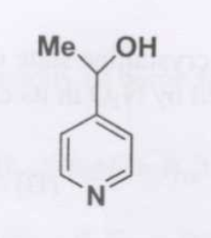
\includegraphics[width=0.1\columnwidth]{figs/q12 c.png}
      \caption{Option C}
    \label{fig:q12 c}
     \item 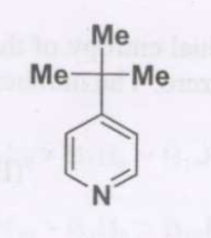
\includegraphics[width=0.1\columnwidth]{figs/q12 d.png}
      \caption{Option D}
    \label{fig:q12 d}
     \end{figure}
\end{enumerate}
   \hfill{\brak{\text{GATE CY 2008}}}


   \item  Cyanogen bromide (CNBr) specifically hydrolyses the peptide bond formed by the C-side of
   \begin{enumerate}
    \begin{multicols}{2}
    \item  methionine  \item  glycine  \item  proline  \item  serine    \hfill{\brak{\text{GATE CY 2008}}}    
    \end{multicols}
\end{enumerate}

    

    \item The Hammett reaction constant $\rho$ is based on
    \begin{enumerate}
    \item  the rates of alkaline hydrolysis of substituted ethyl benzoates
    \item  the dissociation constants of substituted acetic acids
    \item  the dissociation constants of substituted benzoic acids
    \item  the dissociation constants of substituted phenols    \hfill{\brak{\text{GATE CY 2008}}}
    \end{enumerate}


    

    \item The lifetime of a molecule in an excited electronic state is $10^{-10}$ s. The uncertainty in the energy (eV) approximately is
    \begin{enumerate}
    \begin{multicols}{2}
    \item  $2 \times 10^5$  \item  $3 \times 10^6$  \item  0  \item  $10^{-14}$ 
    \end{multicols}
 \hfill{\brak{\text{GATE CY 2008}}}
\end{enumerate}
    

    \item For a one component system, the maximum number of phases that can coexist at equilibrium is
    \begin{enumerate}
    \begin{multicols}{2}
        \item  3  \item  2  \item  1  \item  4    \hfill{\brak{\text{GATE CY 2008}}}
    \end{multicols}
\end{enumerate}
    

    \item At $T = 300 \ \mathrm{K}$, the thermal energy ($k_B T$) in cm\textsuperscript{-1} is approximately
    \begin{enumerate}
\begin{multicols}{2}
        \item  20000  \item  8000  \item  5000  \item  200    \hfill{\brak{\text{GATE CY 2008}}}
\end{multicols}
\end{enumerate}

    

    \item For the reaction $2 X_3 \rightarrow 3 X_2$, the rate of formation of $X_2$ is
\begin{enumerate}

\item $3 \brak{-\frac{d[X_3]}{dt}}$
\item $\frac{1}{2} \brak{-\frac{d[X_3]}{dt}}$
\item $\frac{1}{3} \brak{-\frac{d[X_3]}{dt}}$
\item $\frac{3}{2} \brak{-\frac{d[X_3]}{dt}}$  \hfill{\brak{\text{GATE CY 2008}}}
\end{enumerate}



\item The highest occupied molecular orbital of HF is
\begin{enumerate}
\begin{multicols}{2}
\item  bonding 
\item  antibonding 
\item  ionic 
\item  nonbonding    \hfill{\brak{\text{GATE CY 2008}}} 
\end{multicols}
\end{enumerate}


   \item  The residual entropy of the asymmetric molecule N$_2$O in its crystalline state is $5.8\ \mathrm{J\ K^{-1}\ mol^{-1}}$ at absolute zero. The number of orientations that can be adopted by N$_2$O in its crystalline state is \begin{enumerate}
\begin{multicols}{2}
\item  4 
\item  3 
\item  2 
\item  1    
\end{multicols}
\hfill{\brak{\text{GATE CY 2008}}} 
\end{enumerate}


\textbf{Q.21 to Q.75 Carry two marks each}


\item The spectroscopic ground state symbol and the total number of electronic transitions of [Ti(H$_2$O)$_6$]$^{3+}$ are
\begin{enumerate}
\begin{multicols}{2}
\item  $^3T_{1g}$ and 2 
\item  $^3A_{2g}$ and 3 
\item  $^1T_{1g}$ and 3 
\item  $^3A_{2g}$ and 2    \hfill{\brak{\text{GATE CY 2008}}}
\end{multicols}
\end{enumerate}


\item The structures of the complexes [Cu(NH$_3$)$_4$](ClO$_4$)$_2$ and [Cu(NH$_3$)$_4$](ClO$_4$) in solution respectively are
\begin{enumerate}
\item  square planar and tetrahedral 
\item  octahedral and square pyramidal
\item  octahedral and trigonal bipyramidal 
\item  tetrahedral and square planar    \hfill{\brak{\text{GATE CY 2008}}}
\end{enumerate}


\item In biological systems, the metal ions involved in electron transport are
\begin{enumerate}
\begin{multicols}{2}
\item  Na$^+$ and K$^+$ 
\item  Zn$^{2+}$ and Mg$^{2+}$ 
\item  Ca$^{2+}$ and Mg$^{2+}$ 
\item  Cu$^{2+}$ and Fe$^{3+}$   
\end{multicols}
 \hfill{\brak{\text{GATE CY 2008}}}
\end{enumerate}

\item In a homogeneous catalytic reaction, 1.0 M of a substrate and 1.0 $\mu$M of a catalyst yields 1.0 mM of a product in 10 seconds. The turnover frequency (TOF) of the reaction (s$^{-1}$) is
\begin{enumerate}
\begin{multicols}{2}
\item  $10^2$ 
\item  $10^1$ 
\item  $10^{-3}$ 
\item  $10^3$    
\end{multicols}   \hfill{\brak{\text{GATE CY 2008}}}
\end{enumerate}


\item The expected magnetic moments of the first-row transition metal complexes and those of the lanthanide metal complexes are usually calculated using
\begin{enumerate}
\item  $\mu_{\text{so}}$ equation (s.o. = spin only) for both lanthanide and transition metal complexes
\item  $\mu_{\text{so}}$ equation for lanthanide metal complexes and $\mu$ equation for transition metal complexes
\item  $\mu_{\text{so}}$ equation for transition metal complexes and $\mu$ equation for lanthanide metal complexes
\item  $\mu_{\text{eff}}$ equation for transition metal complexes and $\mu_{\text{so}}$ equation for lanthanide metal complexes    \hfill{\brak{\text{GATE CY 2008}}}
\end{enumerate}




\item The Brønsted acidity of boron hydrides follows the order

\begin{enumerate}
    \item $\mathrm{B_2H_6 > B_4H_{10} > B_5H_9 > B_{10}H_{14}}$
    \item $\mathrm{B_2H_6 = B_4H_{10} > B_5H_9 = B_{10}H_{14}}$
    \item $\mathrm{B_{10}H_{14} > B_5H_9 > B_4H_{10} > B_2H_6}$
    \item $\mathrm{B_5H_9 > B_4H_{10} > B_2H_6 > B_{10}H_{14}}$
\end{enumerate}  \hfill{\brak{\text{GATE CY 2008}}}


\item NaCl is crystallised by slow evaporation of its aqueous solution at room temperature. The correct statement is
\begin{enumerate}
\item  The crystals will be non-stoichiometric
\item  The crystals should have Frenkel defects
\item  The percentage of defects in the crystals will depend on the concentration of the solution and its rate of evaporation
\item  The nature of defects will depend upon the concentration of the solution and its rate of evaporation    \hfill{\brak{\text{GATE CY 2008}}}
\end{enumerate}


\item CaTiO$_3$ has a perovskite crystal structure. The coordination number of titanium in CaTiO$_3$ is
\begin{enumerate}
\begin{multicols}{2}
\item  9 
\item  6 
\item  3 
\item  12   
\end{multicols}
 \hfill{\brak{\text{GATE CY 2008}}}
\end{enumerate}



\item If ClF$_5$ were to be stereochemically rigid, its $^{19}$F NMR spectrum \brak{I for \ensuremath{^{19}\mathrm{F}} = \ensuremath{\frac{1}{2}}}
 would be (assume that Cl is not NMR active)
\begin{enumerate}
\item a doublet and a triplet
\item a singlet
\item  a doublet and a singlet
\item two singlets    \hfill{\brak{\text{GATE CY 2008}}}
\end{enumerate}


\item The point group of NSF$_3$ is
\begin{enumerate}
\begin{multicols}{2}
 \item  D$_{3d}$ 
\item  C$_{3h}$ 
\item  D$_{3h}$ 
\item  C$_{3v}$   
\end{multicols}
    \hfill{\brak{\text{GATE CY 2008}}}
\end{enumerate}

\item When NiO is heated with a small amount of Li$_2$O in air at 1200$^\degree$C, a non-stoichiometric compound Li$_x$Ni$_{1-x}$O is formed. This compound is
\begin{enumerate}
\item  an n-type semiconductor containing only Ni$^{1+}$
\item an n-type semiconductor containing Ni$^{1+}$ and Ni$^{2+}$
\item a p-type semiconductor containing Ni$^{2+}$ and Ni$^{3+}$
\item a p-type semiconductor containing only Ni$^{3+}$    \hfill{\brak{\text{GATE CY 2008}}}
\end{enumerate}
\degree




\item White phosphorus, P$_4$, belongs to the
\begin{enumerate}
\begin{multicols}{4}
\item  \textit{closo} system 
\item  \textit{nido} system 
\item  \textit{arachno} system 
\item  \textit{hypho} system      
\end{multicols}
  \hfill{\brak{\text{GATE CY 2008}}}
\end{enumerate}

\item Among the compounds Fe$_3$O$_4$, NiFe$_2$O$_4$ and Mn$_3$O$_4$
\begin{enumerate}
\item NiFe$_2$O$_4$ and Mn$_3$O$_4$ are normal spinels
\item Fe$_3$O$_4$ and Mn$_3$O$_4$ are normal spinels
\item Fe$_3$O$_4$ and Mn$_3$O$_4$ are inverse spinels
\item Fe$_3$O$_4$ and NiFe$_2$O$_4$ are inverse spinels    \hfill{\brak{\text{GATE CY 2008}}}
\end{enumerate}

\item The number of M-M bonds in Ir$_4$(CO)$_{12}$ are
\begin{enumerate}
\begin{multicols}{2}
\item  four 
\item  six 
\item  eight 
\item  zero     
\end{multicols}
   \hfill{\brak{\text{GATE CY 2008}}}
\end{enumerate}

\item Schrock carbenes are
\begin{enumerate}
\begin{multicols}{2}
\item  triplets and nucleophilic 
\item  triplets and electrophilic
\item  singlets and nucleophilic 
\item  singlets and electrophilic
\end{multicols}
\hfill{\brak{\text{GATE CY 2008}}}
\end{enumerate}


\item The \textbf{INCORRECT} statement about linear dimethylpolysiloxane, [(CH$_3$)$_2$SiO]$_n$, is
\begin{enumerate}
\item it is extremely hydrophilic
\item it is prepared by a KOH catalysed ring-opening reaction of [Me$_2$SiO]$_4$
\item it has a very low glass transition temperature
\item it can be reinforced to give silicon elastomers    \hfill{\brak{\text{GATE CY 2008}}}

\end{enumerate}




\item Match the entries \textbf{a–d} with their corresponding structures \textbf{p–s}

\begin{figure}[H]]
    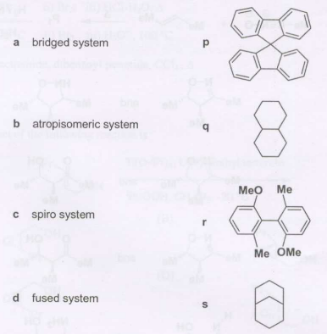
\includegraphics[width=0.8\columnwidth]{figs/q37.png}
\caption{Figure for Q.37}
    \label{fig:q37}
\end{figure}
\begin{enumerate}
    \item a - s, b - r, c - q, d - p
    \item a - p, b - s, c - q, d - r
    \item a - q, b - p, c - s, d - r
    \item a - s, b - r, c - p, d - q
\end{enumerate}    \hfill{\brak{\text{GATE CY 2008}}}


\item The reaction between \textbf{X} and \textbf{Y} to give \textbf{Z} proceeds via

\begin{figure}[H]
    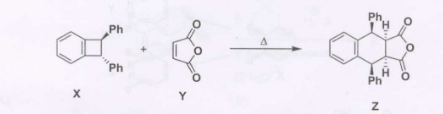
\includegraphics[width=0.8\columnwidth]{figs/q38.png}
    \caption{Figure for Q.38}
    \label{fig:q38}
\end{figure}
\begin{enumerate}
    \item $4\pi$-conrotatory opening of X followed by \textit{endo} Diels--Alder cycloaddition
    \item $4\pi$-disrotatory opening of X followed by \textit{endo} Diels--Alder cycloaddition
    \item $4\pi$-conrotatory opening of X followed by \textit{exo} Diels--Alder cycloaddition
    \item  $4\pi$-disrotatory opening of X followed by \textit{exo} Diels--Alder cycloaddition
\end{enumerate}    \hfill{\brak{\text{GATE CY 2008}}}


\item The major products $P_1$ and $P_2$, respectively, in the following reaction sequence are

\begin{figure}[H]
    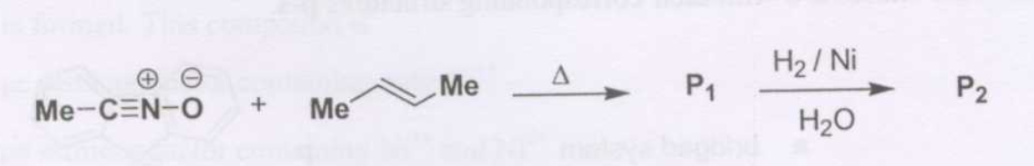
\includegraphics[width=0.5\columnwidth]{figs/q39.png}
    \caption{Figure for Q.39}
    \label{fig:q39}
\end{figure}    \hfill{\brak{\text{GATE CY 2008}}}
\begin{enumerate}
\begin{figure}[H]
    \item 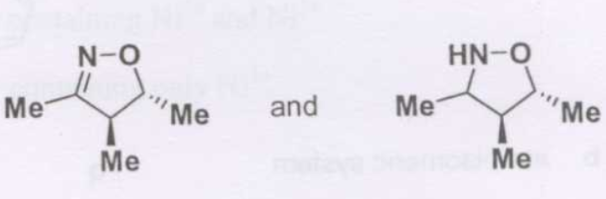
\includegraphics[width=0.3\columnwidth]{figs/q39 a.png}
    \caption{Option A}
    \label{fig:q39 a}
    \item 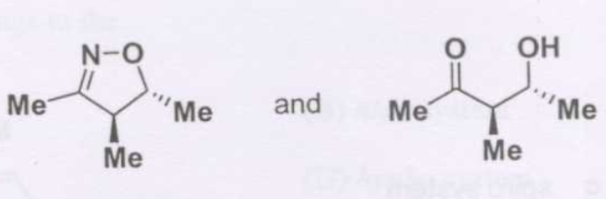
\includegraphics[width=0.3\columnwidth]{figs/q39 b.png}
    \caption{Option B}
    \label{fig:q39 b}
    \item 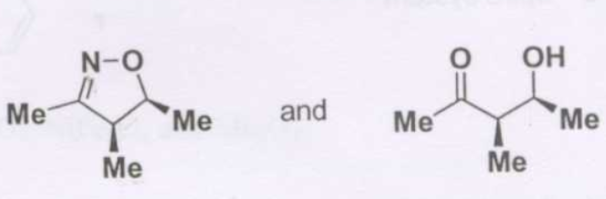
\includegraphics[width=0.3\columnwidth]{figs/q39 c.png}
    \caption{Option C}
    \label{fig:q39 c}
    \item 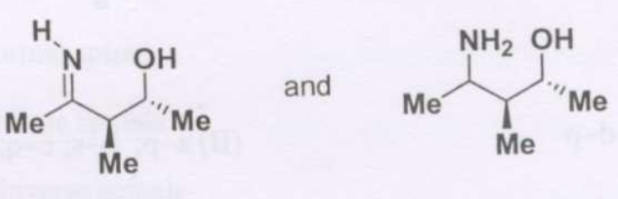
\includegraphics[width=0.3\columnwidth]{figs/q39 d.png}
    \caption{Option D}
    \label{fig:q39 d}
    \end{figure}
\end{enumerate}

\item The products $Y$ and $Z$ are formed, respectively, from $X$ via

\begin{figure}[H]
    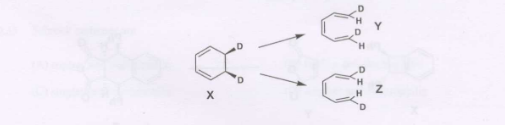
\includegraphics[width=0.8\columnwidth]{figs/q40.png}
     \caption{Figure for Q.40}
    \label{fig:q40}
\end{figure}
\begin{enumerate}
    \item $h\nu$, conrotatory opening and $\Delta$, disrotatory opening
    \item $h\nu$, disrotatory opening and $\Delta$, conrotatory opening
    \item $\Delta$, conrotatory opening and $h\nu$, disrotatory opening
    \item $\Delta$, disrotatory opening and $h\nu$, conrotatory opening
\end{enumerate}    \hfill{\brak{\text{GATE CY 2008}}}



\item \textit{o}-Bromophenol is readily prepared from phenol using the following conditions:
\begin{enumerate}
\item i) (CH$_3$CO)$_2$O;  ii) Br$_2$;  iii) HCl–H$_2$O, $\Delta$
\item i) H$_2$SO$_4$, 100$^\degree$C;  ii) Br$_2$;  iii) H$_3$O$^+$, 100$^\degree$C
\item N-Bromosuccinimide, dibenzoyl peroxide, CCl$_4$, $\Delta$
\item Br$_2$/FeBr$_3$    \hfill{\brak{\text{GATE CY 2008}}}
\end{enumerate}


\item The major product of the following reaction is

\begin{figure}[H]
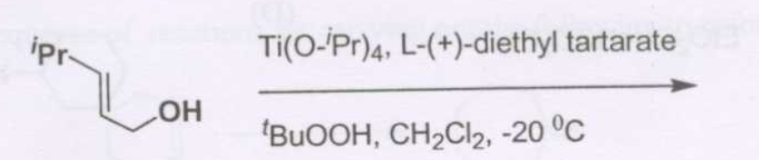
\includegraphics[width=0.6\columnwidth]{figs/q42.png}
\caption{Figure for Q.42}
    \label{fig:q42}
\end{figure}    \hfill{\brak{\text{GATE CY 2008}}}
\begin{enumerate}
\begin{figure}[H]
    \item 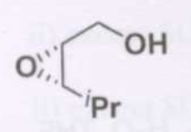
\includegraphics[width=0.2\columnwidth]{figs/q42 a.png} 
    \caption{Option A}
    \label{fig:q42 a}
    \item 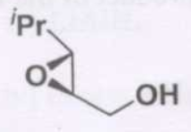
\includegraphics[width=0.2\columnwidth]{figs/q42 b.png} 
    \caption{Option B}
    \label{fig:q42 b}
    \item 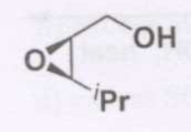
\includegraphics[width=0.2\columnwidth]{figs/q42 c.png} 
    \caption{Option C}
    \label{fig:q42 c}
    \item 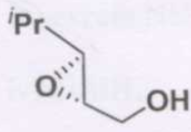
\includegraphics[width=0.2\columnwidth]{figs/q42 d.png} 
    \caption{Option D}
    \label{fig:q42 d}
    \end{figure}
\end{enumerate}

\item The photochemical reaction of 2-methylpropane with F$_2$ gives 2-fluoro-2-methylpropane and 1-fluoro-2-methylpropane in 14:86 ratio. The corresponding ratio of the bromo products in the above reaction using Br$_2$ is most likely to be:
\begin{enumerate}
\item 14 : 86
\item 50 : 50
\item 1 : 9
\item 99 : 1    
\end{enumerate}
\hfill{\brak{\text{GATE CY 2008}}}


\item The major product $P$ of the following reaction is

\begin{figure}[H]
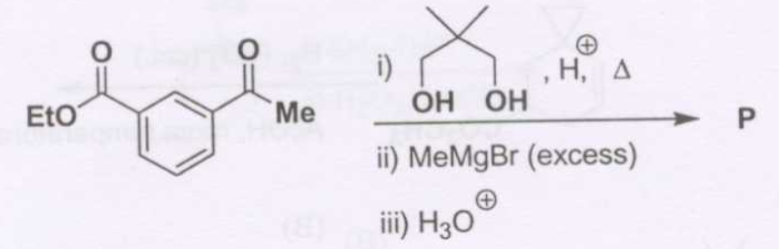
\includegraphics[width=0.6\columnwidth]{figs/q44.png}
\caption{Figure for Q.44}
    \label{fig:q44}
\end{figure}    \hfill{\brak{\text{GATE CY 2008}}}
\begin{enumerate}
\begin{figure}[H]
    \item 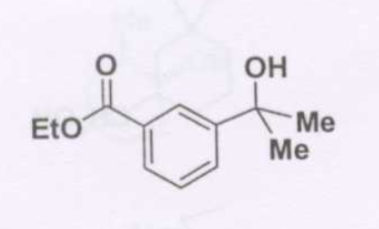
\includegraphics[width=0.2\columnwidth]{figs/q44 a.png}
    \caption{Option A}
    \label{fig:q44 a}
    \item 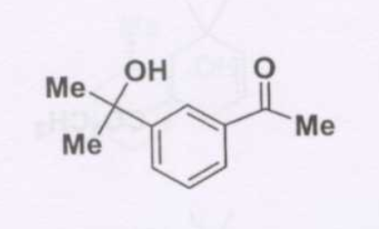
\includegraphics[width=0.2\columnwidth]{figs/q44 b.png}
    \caption{Option B}
    \label{fig:q44 b}
    \item 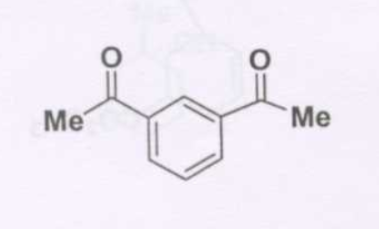
\includegraphics[width=0.2\columnwidth]{figs/q44 c.png}
    \caption{Option C}
    \label{fig:q44 c}
    \item 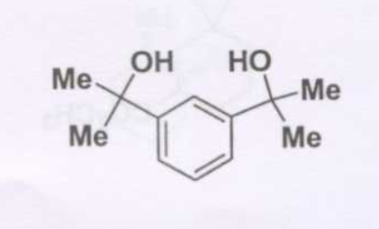
\includegraphics[width=0.2\columnwidth]{figs/q44 d.png}
    \caption{Option D}
    \label{fig:q44 d}
    \end{figure}
\end{enumerate}


\item The reagent \textbf{X} in the following reaction is

\begin{figure}[H]
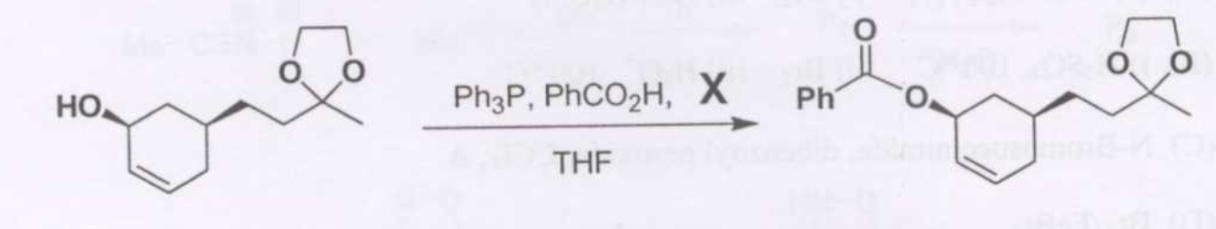
\includegraphics[width=0.6\columnwidth]{figs/q45.png}
\caption{Figure for Q.45}
    \label{fig:q45}
\end{figure}    \hfill{\brak{\text{GATE CY 2008}}}
\begin{enumerate}
\item HO$_2$CN=NCO$_2$H
\item EtO$_2$CHC=CH-CO$_2$Et
\item EtO$_2$CN=NCO$_2$Et
\begin{figure}[H]
\item 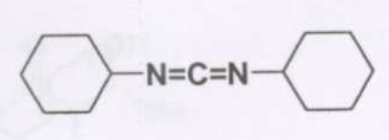
\includegraphics[width=0.3\columnwidth]{figs/q45 d.png}
\caption{Option D}
    \label{fig:q45 d}
\end{figure}
\end{enumerate}


\item The major product of the following reactions is

\begin{figure}[H]
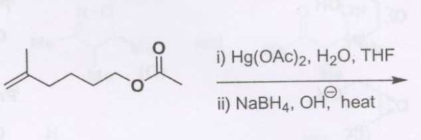
\includegraphics[width=0.6\columnwidth]{figs/q46.png}
\caption{Figure for Q.46}
    \label{fig:q46}
\end{figure}    \hfill{\brak{\text{GATE CY 2008}}}
\begin{enumerate}
\begin{figure}[H]
    \item 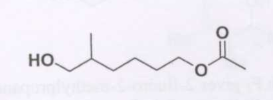
\includegraphics[width=0.3\columnwidth]{figs/q46 a.png}
    \caption{Option A}
    \label{fig:q46 a}
    \item 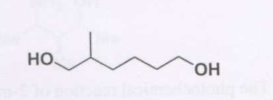
\includegraphics[width=0.3\columnwidth]{figs/q46 b.png}
    \caption{Option B}
    \label{fig:q46 b}
    \item 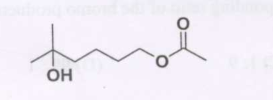
\includegraphics[width=0.3\columnwidth]{figs/q46 c.png}
    \caption{Option C}
    \label{fig:q46 c}
    \item 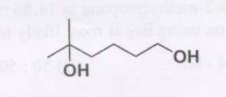
\includegraphics[width=0.3\columnwidth]{figs/q46 d.png}
    \caption{Option D}
    \label{fig:q46 d}
    \end{figure}
\end{enumerate}


\item The major product of the following reaction is

\begin{figure}[H]
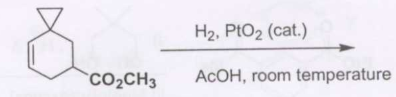
\includegraphics[width=0.6\columnwidth]{figs/q47.png}
\caption{Figure for Q.47}
    \label{fig:q47}
\end{figure}    \hfill{\brak{\text{GATE CY 2008}}}
\begin{enumerate}
\begin{figure}[H]
    \item 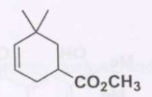
\includegraphics[width=0.3\columnwidth]{figs/q47 a.png}
    \caption{Option A}
    \label{fig:q47 a}
    \item 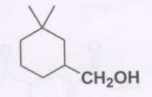
\includegraphics[width=0.3\columnwidth]{figs/q47 b.png}
    \caption{Option B}
    \label{fig:q47 b}
    \item 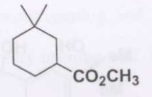
\includegraphics[width=0.3\columnwidth]{figs/q47 c.png}
    \caption{Option C}
    \label{fig:q47 c}
    \item 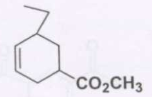
\includegraphics[width=0.3\columnwidth]{figs/q47 d.png}
    \caption{Option D}
    \label{fig:q47 d}
    \end{figure} 
\end{enumerate}

\item In the following compound, the hydroxy group that is most readily methylated with CH$_2$N$_2$ is

\begin{figure}[H]
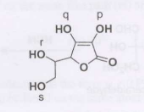
\includegraphics[width=0.45\columnwidth]{figs/q48.png}
\caption{Figure for Q.48}
    \label{fig:q48}
\end{figure}
\begin{enumerate}
\begin{multicols}{2}
 \item  p \item  q  \item  r  \item  s
\end{multicols}
     \hfill{\brak{\text{GATE CY 2008}}}
\end{enumerate}

\item The most appropriate sequence of reactions for carrying out the following transformation is

\begin{figure}[H]
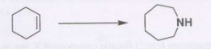
\includegraphics[width=0.45\columnwidth]{figs/q49.png} 
\caption{Figure for Q.49}
    \label{fig:q49}
\end{figure}

\begin{enumerate}
\item i) O$_3$/H$_2$O$_2$;  ii) excess SOCl$_2$/pyridine;  iii) excess NH$_3$;  iv) LiAlH$_4$ 
\item i) O$_3$/Me$_2$S;  ii) excess SOCl$_2$/pyridine;  iii) LiAlH$_4$;  iv) excess NH$_3$ 
\item i) O$_3$/H$_2$O$_2$;  ii) excess SOCl$_2$/pyridine;  iii) LiAlH$_4$;  iv) excess NH$_3$ 
\item  i) O$_3$/Me$_2$S;  ii) excess SOCl$_2$/pyridine;  iii) excess NH$_3$;  iv) LiAlH$_4$ 
\end{enumerate}    \hfill{\brak{\text{GATE CY 2008}}}


\item The number of optically active stereoisomers possible for 1,3-cyclohexanediol in its chair conformation is
\begin{enumerate}
\item 4
\item 3
\item 2
\item 1    \hfill{\brak{\text{GATE CY 2008}}}
\end{enumerate}



\item The major product of the following reactions is

\begin{figure}[H]
\includegraphics[width=0.6\columnwidth]{figs/q51.png}
\caption{Figure for Q.51}
\end{figure}    
\begin{enumerate}
\begin{figure}[H]
    \item \includegraphics[width=0.2\columnwidth]{figs/q51 a.png}
    \caption{Option A}
    \label{fig:q51 a}
    \item \includegraphics[width=0.2\columnwidth]{figs/q51 b.png}
    \caption{Option B}
    \label{fig:q51 b}
    \item \includegraphics[width=0.2\columnwidth]{figs/q51 c.png}
    \caption{Option C}
    \label{fig:q51 c}
    \item \includegraphics[width=0.2\columnwidth]{figs/q51 d.png}
    \caption{Option D}
    \label{fig:q51 d}
    \end{figure}  \hfill{\brak{\text{GATE CY 2008}}}
\end{enumerate}

\item In the folloowing reaction,

\begin{figure}[H]
\includegraphics[width=0.6\columnwidth]{figs/q52.png}
\caption{Figure for Q.52}
    \label{fig:q52}
\end{figure}

 The absolute configurations of the chiral centres in X and Y are

\begin{enumerate}
\item  2S, 3R  and  2R, 3R 
\item  2R, 3R  and  2R, 3S 
\item  2S, 3S  and  2R, 3R 
\item  2S, 3R  and  2S, 3R
\end{enumerate}    \hfill{\brak{\text{GATE CY 2008}}}


\item The IR stretching frequencies (cm$^{-1}$) for the compound X are as follows: 3300--3500 (s, br); 3000 (m); 2225 (s); 1680 (s). 

\begin{figure}[H]
\includegraphics[width=0.6\columnwidth]{figs/q53.png}
\caption{Figure for Q.53}
    \label{fig:q53}
\end{figure}

The correct assignment of the absorption bands is:

\begin{enumerate}
\item  $\bar{\nu}_{\text{OH}} = 3300$--$3500$; $\bar{\nu}_{\text{CH}} = 3000$; $\bar{\nu}_{\text{CN}} = 2225$; $\bar{\nu}_{\text{CO}} = 1680$ 
\item  $\bar{\nu}_{\text{OH}} = 3000$; $\bar{\nu}_{\text{CH}} = 3300$--$3500$; $\bar{\nu}_{\text{CN}} = 2225$; $\bar{\nu}_{\text{CO}} = 1680$ 
\item  $\bar{\nu}_{\text{OH}} = 3300$--$3500$; $\bar{\nu}_{\text{CH}} = 3000$; $\bar{\nu}_{\text{CN}} = 1680$; $\bar{\nu}_{\text{CO}} = 2225$ 
\item  $\bar{\nu}_{\text{OH}} = 3000$; $\bar{\nu}_{\text{CH}} = 3300$--$3500$; $\bar{\nu}_{\text{CN}} = 1680$; $\bar{\nu}_{\text{CO}} = 2225$
\end{enumerate}    \hfill{\brak{\text{GATE CY 2008}}}


\item The T$_d$ point group has 24 elements and 5 classes. Given that it has two 3-dimensional irreducible representations, the number of one-dimensional irreducible representations is
\begin{enumerate}
\begin{multicols}{2}
\item  1
\item  6
\item  2
\item  3    \hfill{\brak{\text{GATE CY 2008}}}
\end{multicols}
\end{enumerate}

\item The total number of ways in which two nonidentical spin $\frac{1}{2}$ particles can be oriented relative to a constant magnetic field is
\begin{enumerate}
\begin{multicols}{2}
\item  1
\item  2
\item  3
\item  4    \hfill{\brak{\text{GATE CY 2008}}}
\end{multicols}
\end{enumerate}


\item Approximately one hydrogen atom per cubic meter is present in interstellar space. Assuming that the H-atom has a diameter of $10^{-10}$ m, the mean free path (m) approximately is
\begin{enumerate}
\begin{multicols}{4}
    
\item  $10^{10}$
\item  $10^{19}$
\item  $10^{24}$
\item  $10^{14}$
\end{multicols}    \hfill{\brak{\text{GATE CY 2008}}}
\end{enumerate}

\item The wavefunction of a diatomic molecule has the form $\psi = 0.89\, \varphi_{\text{covalent}} + 0.45\, \varphi_{\text{ionic}}$. The chance that both electrons of the bond will be found on the same atom in 100 inspections of the molecule approximately is

\begin{enumerate}
\item 79
\item 20
\item 45
\item 60
\end{enumerate}    \hfill{\brak{\text{GATE CY 2008}}}




\item For the reaction given below, the relaxation time is $10^{-4}$ s. Given that 10\% of A remains at equilibrium, the value of $k_1$ (s$^{-1}$) is

\begin{figure}[H]
\includegraphics[width=0.3\columnwidth]{figs/q58.png}
\caption{Figure for Q.58}
    \label{fig:q58}
\end{figure}

\begin{enumerate}
\item $9 \times 10^5$
\item $10^5$
\item $10^6$
\item $9 \times 10^6$
\end{enumerate}    \hfill{\brak{\text{GATE CY 2008}}}




\item The minimum number of electrons needed to form a chemical bond between two atoms is

\begin{enumerate}
\item 1
\item 2
\item 3
\item 4
\end{enumerate}    \hfill{\brak{\text{GATE CY 2008}}}




\item The ground state electronic energy (Hartree) of a helium atom, neglecting the inter-electron repulsion, is

\begin{enumerate}
\item -1.0
\item -0.5
\item -2.0
\item -4.0
\end{enumerate}    \hfill{\brak{\text{GATE CY 2008}}}




\item A particle is confined to a one-dimensional box of length 1 mm. If the length is changed by $10^{-9}$ m, the \% change in the ground state energy is

\begin{enumerate}
\item $2 \times 10^4$
\item $2 \times 10^7$
\item $2 \times 10^2$
\item 0
\end{enumerate}    \hfill{\brak{\text{GATE CY 2008}}}




\item A certain molecule can be treated as having only a doubly degenerate state lying at 360 cm$^{-1}$ above the nondegenerate ground state. The approximate temperature (K) at which 15\% of the molecules will be in the upper state is

\begin{enumerate}
\item 500
\item 150
\item 200
\item 300
\end{enumerate}    \hfill{\brak{\text{GATE CY 2008}}}




\item A box of volume $V$ contains one mole of an ideal gas. The probability that all $N$ particles will be found occupying one half of the volume leaving the other half empty is

\begin{enumerate}
\item $1/2$
\item $2/N$
\item $(1/2)^N$
\item $(1/2)^{6N}$
\end{enumerate}    \hfill{\brak{\text{GATE CY 2008}}}




\item According to the Debye-Hückel limiting law, the mean activity coefficient of $5 \times 10^{-4}~\text{mol kg}^{-1}$ aqueous solution of CaCl$_2$ at 25$^\degree$C is (the Debye-Hückel constant ‘A’ can be taken to be 0.509)

\begin{enumerate}
\item 0.63
\item 0.72
\item 0.80
\item 0.91
\end{enumerate}    \hfill{\brak{\text{GATE CY 2008}}}




\item The operation of the commutator \brak{ x, \brak{\frac{d}{dx}} }
 on a function $f(x)$ is equal to

\begin{enumerate}
\item 0
\item $f(x)$
\item $-f(x)$
\item $x \frac{df}{dx}$
\end{enumerate}    \hfill{\brak{\text{GATE CY 2008}}}




\item If a gas obeys the equation of state $P (V - nb) = nRT$, the ratio $(C_P - C_V)/(C_P - C_V)_{\text{ideal}}$ is

\begin{enumerate}
\item $> 1$
\item $< 1$
\item 1
\item $(1 - b)$
\end{enumerate}    \hfill{\brak{\text{GATE CY 2008}}}




\item Physisorbed particles undergo desorption at 27$^\degree$C with an activation energy of 16.628 kJ mol$^{-1}$. Assuming first-order process and a frequency factor of $10^{12}$ Hz, the average residence time (in seconds) of the particles on the surface is

\begin{enumerate}
\item $8 \times 10^{-10}$
\item $8 \times 10^{-11}$
\item $2 \times 10^{-9}$
\item $1 \times 10^{-12}$
\end{enumerate}    \hfill{\brak{\text{GATE CY 2008}}}




\item The rotational constants for CO in the ground and the first excited vibrational states are 1.9 and 1.6 cm$^{-1}$, respectively. The \% change in the internuclear distance due to vibrational excitation is

\begin{enumerate}
\item 9
\item 30
\item 16
\item 0
\end{enumerate}    \hfill{\brak{\text{GATE CY 2008}}}




\item
The mechanism of enzyme (E) catalysed reaction of a substrate (S) to yield product (P) is:

\begin{figure}[H]
\includegraphics[width=0.6\columnwidth]{figs/q69.png}
\caption{Figure for Q.69}
    \label{fig:q69}
\end{figure}

If a small amount of S is converted to P, the maximum rate for the reaction will be observed for:

\begin{enumerate}
\item   $(k_1 + k_2) \gg k_1 [S]_0$
\item   $(k_1 + k_2) \ll k_1 [S]_0$ 
\item   $(k_2 + k_{-1}) = (k_1 + k_1)$ 
\item   $k_2 \ll k_1$
\end{enumerate}    \hfill{\brak{\text{GATE CY 2008}}}


\item The lowest energy state of the $(1s)^2(2s)^1(3s)^1$ configuration of Be is

\begin{enumerate}
\item $^1S_0$
\item $^1D_2$
\item $^3S_1$
\item $^3P_1$
\end{enumerate}    \hfill{\brak{\text{GATE CY 2008}}}



\section*{Common Data Questions}

{Common Data for Questions 71, 72 and 73:} 
An electron accelerated through a potential difference of $\varphi$ volts impinges on a nickel surface, whose \brak{100} planes have a spacing $d = 351.8 \times 10^{-12}$ m \brak{351.8 pm}.


    \item The de-Broglie wavelength of the electron is $\lambda/\text{pm} = \brak{a/\varphi}^{1/2}$. The value of ‘a’ in volts is:
    \begin{enumerate}
        \item $1.5 \times 10^{-18}$
        \item $1.5 \times 10^6$
        \item $6.63 \times 10^5$
        \item $2.5 \times 10^{18}$
    \end{enumerate}    \hfill{\brak{\text{GATE CY 2008}}}


    \item The condition for observing diffraction from the nickel surface is:
    \begin{enumerate}
        \item $\lambda \gg 2d$
        \item $\lambda \leq 2d$
        \item $\lambda \leq d$
        \item $\lambda \geq d$
    \end{enumerate}    \hfill{\brak{\text{GATE CY 2008}}}


    \item The minimum value of $\varphi$ (V) for the electron to diffract from the \brak{100} planes is:
    \begin{enumerate}
        \item 3000
        \item 300
        \item 30
        \item 3
    \end{enumerate}
    \hfill{\brak{\text{GATE CY 2008}}}


{Common Data for Questions 74 and 75:} 
An iron complex $[\text{FeL}_3]^{2+}$ (L = neutral monodentate ligand) catalyses the oxidation of (CH$_3$)$_2$S by perbenzoic acid.


    \item The formation of the organic product in the above reaction can be monitored by:
    \begin{enumerate}
        \item gas chromatography
        \item cyclic voltammetry
        \item electron spin resonance
        \item fluorescence spectroscopy
    \end{enumerate}    \hfill{\brak{\text{GATE CY 2008}}}


    \item The oxidation state of the metal ion in the catalyst can be detected by:
    \begin{enumerate}
        \item atomic absorption spectroscopy
        \item M\"ossbauer spectroscopy
        \item HPLC
        \item gas chromatography
    \end{enumerate}
  \hfill{\brak{\text{GATE CY 2008}}}


\section{Linked Answer Questions: Q.76 to Q.85 carry two marks each}

{Linked Answer Questions 76 and 77:}

In the reaction,

\begin{figure}[H]
\includegraphics[width=0.6\columnwidth]{figs/q76 1.png}
\caption{Figure for Q.76}
    \label{fig:q76 1}
\end{figure} 


\item Compound $X$ is

\begin{enumerate}
\begin{figure}[H]
\item \includegraphics[width=0.2\columnwidth]{figs/q76 a.png}
\caption{Option A}
    \label{fig:q76 a}
\item \includegraphics[width=0.2\columnwidth]{figs/q76 b.png}
\caption{Option B}
    \label{fig:q76 b}
\item \includegraphics[width=0.2\columnwidth]{figs/q76 c.png}
\caption{Option C}
    \label{fig:q76 c}
\item \includegraphics[width=0.2\columnwidth]{figs/q76 d.png}
\caption{Option D}
    \label{fig:q76 d}
\end{figure}
\end{enumerate}    \hfill{\brak{\text{GATE CY 2008}}}


\item Rh(PPh$_3$)$_3$Cl reacts very fast with a gaseous mixture of H$_2$ and C$_2$H$_4$ to immediately give $Z$.The structure of $Z$ is

\begin{enumerate}
\begin{figure}[H]
\item H$_3$C-CH$_3$
\item \includegraphics[width=0.3\columnwidth]{figs/q77 b.png}
\caption{Option B}
    \label{fig:q77 b}
\item \includegraphics[width=0.3\columnwidth]{figs/q77 c.png}
\caption{Option C}
    \label{fig:q77 c}
\item \includegraphics[width=0.3\columnwidth]{figs/q77 d.png}
\caption{Option D}
    \label{fig:q77 d}
\end{figure}
\end{enumerate}    \hfill{\brak{\text{GATE CY 2008}}}


\section*{Linked Answer Questions 78 and 79}

The reaction of PCl$_3$ with methanol in the presence of triethylamine affords compound X. EI mass spectrum of X shows a parent ion peak at $m/z = 124$. Microanalysis of X shows that it contains C, H, O and P. The $^1$H NMR spectrum of X shows a doublet at 4.0 ppm. The separation between the two lines of the doublet is approximately 15 Hz \brak{J for \ensuremath{^{1}\mathrm{H}}\ and \ensuremath{^{31}\mathrm{P}} = \ensuremath{\tfrac{1}{2}}}.



    \item Compound X is:
    \begin{enumerate}
        \item (CH$_3$O)$_2$P
        \item (CH$_3$O)$_2$PO
        \item (CH$_3$O)$_2$P(O)OH
        \item (CH$_3$O)$_2$PH
    \end{enumerate}    \hfill{\brak{\text{GATE CY 2008}}}


    \item Upon heating, compound X is converted to Y, which has the same molecular formula as that of X. The $^1$H NMR spectrum of Y shows two doublets centered at 3.0 ppm (separation of two lines = 20 Hz) and 4.0 ppm (separation of two lines = 15 Hz) respectively.

    Compound Y is:
    \begin{enumerate}
        \item (CH$_3$O)$_2$P(O)(OH)
        \item (CH$_3$O)$_2$P
        \item (CH$_3$O)(CH$_3$)P(O)
        \item (CH$_3$O)(CH$_3$)P(OH)
    \end{enumerate}
   \hfill{\brak{\text{GATE CY 2008}}}


\section*{Linked Answer Questions 80 and 81}

For butyrophenone (\texttt{PhCOCH\(_2\)CH\(_2\)CH\(_3\)}),

\item  The most probable fragmentation observed in the electron impact ionization (EI) mass spectrometry is

\begin{enumerate}
\begin{figure}[H]
\item \includegraphics[width=0.3\columnwidth]{figs/q80 a.png}
\caption{Option A}
    \label{fig:q80 a}
\item \includegraphics[width=0.3\columnwidth]{figs/q80 b.png}
\caption{Option B}
    \label{fig:q80 b}
\item \includegraphics[width=0.3\columnwidth]{figs/q80 c.png}
\caption{Option C}
    \label{fig:q80 c}
\item \includegraphics[width=0.3\columnwidth]{figs/q80 d.png}
\caption{Option D}
    \label{fig:q80 d}

\end{figure}
\end{enumerate}    \hfill{\brak{\text{GATE CY 2008}}}


\item  Photoirradiation leads to the following set of products.

\begin{enumerate}
\begin{figure}[H]
\item \includegraphics[width=0.3\columnwidth]{figs/q81 a.png}
\caption{Option A}
    \label{fig:q81 a}
\item \includegraphics[width=0.3\columnwidth]{figs/q81 b.png}
\caption{Option B}
    \label{fig:q81 b}
\item \includegraphics[width=0.3\columnwidth]{figs/q81 c.png}
\caption{Option C}
    \label{fig:q81 c}
\item \includegraphics[width=0.3\columnwidth]{figs/q81 d.png}
\caption{Option D}
    \label{fig:q81 d}
\end{figure}
\end{enumerate}     \hfill{\brak{\text{GATE CY 2008}}}


{Linked Answer Questions 82 and 83:}

In the following reaction,

\begin{figure}[H]
\includegraphics[width=0.6\columnwidth]{figs/q82 1.png}
\caption{Figure for Q.82}
    \label{fig:q82}
\end{figure}

\item the reactive intermediate $I$ and the product $P$ are

\begin{enumerate}
\begin{figure}[H]
\item \includegraphics[width=0.3\columnwidth]{figs/q82 a.png}
\caption{Option A}
    \label{fig:q82 a}
\item \includegraphics[width=0.3\columnwidth]{figs/q82 b.png}
\caption{Option B}
    \label{fig:q82 b}
\item \includegraphics[width=0.3\columnwidth]{figs/q82 c.png}
\caption{Option C}
    \label{fig:q82 c}
\item \includegraphics[width=0.3\columnwidth]{figs/q82 d.png}
\caption{Option D}
    \label{fig:q82 d}
\end{figure}
\end{enumerate}     \hfill{\brak{\text{GATE CY 2008}}}


\item The product P shows ‘m’ and ‘n’ number of signals in $^1$H and $^{13}$C NMR spectra, respectively. The values of ‘m’ and ‘n’ are
\begin{enumerate}
\item m= 3 and n = 2
\item m = 2 and n = 3
\item m= 2 and n = 2
\item m = 4 and n = 3
   \hfill{\brak{\text{GATE CY 2008}}}
   \end{enumerate}

    

Linked Answer Questions 84 and 85:

The infrared spectrum of a diatomic molecule exhibits transitions at 2144, 4262 and 6354~cm $^{-1}$ 
corresponding to excitations from the ground state to the first, second, and third vibration states respectively.

\item  The fundamental transition (cm$^{-1}$) of the diatomic molecule is at
\begin{enumerate}
\begin{multicols}{4}
\item  2157  \item  2170 
\item  2183  \item  2196 
\end{multicols}   \hfill{\brak{\text{GATE CY 2008}}}
\end{enumerate}

\item  The anharmonicity constant (cm$^{-1}$) of the diatomic molecule is
\begin{enumerate}
\begin{multicols}{2}
\item  0.018  \item  0.012 
\item  0.006  \item  0.003 
\end{multicols}   \hfill{\brak{\text{GATE CY 2008}}}
\end{enumerate}

\begin{center}
\textbf{END OF THE QUESTION PAPER}
\end{center}

\end{enumerate}
\end{document}
